\documentclass[hyperref, UTF8, cs4size, titlepage]{ctexart}

% 版面制作
\usepackage[a4paper, left=2.5cm, right=2.5cm, top=2.5cm, bottom=2.5cm]{geometry}
% 页面(页尾设置)
\pagestyle{plain}

% 目录拓展
\usepackage[nottoc]{tocbibind}
% 超文本链接设置
\usepackage{bookmark}
\hypersetup{colorlinks=true, linkcolor=blue, filecolor=magenta, urlcolor=cyan, pdfpagemode=FullScreen}

% 引用设置
\bibliographystyle{NCEPU}
% 索引设置
\usepackage{makeidx}
\makeindex
% 附件添加
\usepackage{attachfile}

% 标题设置
\usepackage[tiny, raggedright]{titlesec}
\titleformat*{\section}{\zihao{4}\upshape\bfseries\centering}

% 行距设置
%\usepackage{setspace}
%\setstretch{1}

% 数学
\usepackage{amsmath}

% 代码
\usepackage{listings}

% 图表
\usepackage{caption} % 图表标题
\usepackage{graphicx} % 图片
\usepackage{booktabs} % 三线表
\usepackage{array} % 表格列格式拓展
\usepackage{tikz} % 结构图

% 自定义命令
\newcommand{\keywords}[1]{\textbf{\textit{关键字---}} #1}

\begin{document}

  % 添加封面
  \begin{titlepage}
  \begin{center}
    \vspace*{\fill}
    {\zihao{3}\bfseries 选题:A}
    \vspace*{\fill}

    {\zihao{3}\bfseries 论文题目:}
    \vspace*{\stretch{2}}

    \zihao{4}\itshape
    \begin{tabular}{ccc}
      建模:& 成宇琛 & 电气 1813 班 \\
      编程:& 孙瑞 & 计算机 1806班 \\
      论文:& 邓思彤 & 电气 1813 班 \\
    \end{tabular}
    \vspace*{\stretch{3}}

    \today
  \end{center}
  \vspace*{\stretch{1}}
\end{titlepage}

  % 添加摘要
  \phantomsection
  \begin{abstract}
  \thispagestyle{plain}

  碳排放问题在我国已引起广泛的关注。为对我国实施碳排放减排政策和低碳经济发展战略提供决策依据和有效建议。现对外来几年的碳排放进行预测,并以此提供有效建议。

  \textbf{针对问题一:}
  
  本文做出了了煤炭、石油、天然气和一次电力及其他能源占我国能源消费整体的比重随年份变化的折线图。

  以此为依据展开对我国能源消费结构的分析。分析包括了沿y轴(能源所占比例)和沿x轴(年份变化)的大小与趋势的分析。

  最终得出了:我国能源结构以化石能源(煤炭尤其)为其始终主导的现状;和总体能源结构在不断优化,但仍有相当大发展空间的未来趋势。

  \textbf{针对问题二:}
  
  本文选取、整理了总人口数、$\mathrm{GDP}$、产业结构、城镇化率、经济发展水平、国际贸易、人均碳排放量、能源消费强度,共八个因素作为主要影响因素,并以此建立了\textbf{ $\mathrm{BP}$ 神经网络模型}。

  具体来说:

  本文首先对样本数据进行计算、分类和归一化处理。再确定模型输出层、中间隐层和输入层,以及具体函数、参数选取、初始化。

  之后借助于 $\mathrm{MATLAB}$ 软件中的神经网络计算功能,对模型进行了合理训练和数据拟合。最终得到对应年份的碳排放量的模拟值和预测值。

  \textbf{针对问题三:}
  
  本文首先在\emph{模型评价与改进}中应用\textbf{关联度分析法}建立了\textbf{灰色关联模型}。
  
  之后代入数据到关联系数公式中,得出影响因素数列对参考数列的关联度,以此对各影响因素进行了关联性排序。

  通过关联度大小排序也就得到了影响因素的重要性排序。其结果是:$\text{总人口数}>\mathrm{GDP}>\text{其他}$。其中,总人口数和$\mathrm{GDP}$ 关联度徘徊在 0.6 上下,其他值集中在 0.39 上下。

  最终我们根据影响因素的重要性,提出:
  \begin{enumerate}
    \item 加快中国 $\mathrm{GDP}$ 由高速度增长向高质量发展的经济转型。
    \item 坚持计划生育的基本国策。
    \item 转移城市过剩生产力,帮助农村发展,减少城乡差异。
    \item 寻求开发绿色能源、新能源,减少对化石能源的依赖。
  \end{enumerate}

  \vspace{\stretch{3}}
  {\keywords{碳排放,能源结构,$\mathrm{BP}$ 神经网络,灰色关联模型,关联度分析法}}
  \vspace{\fill}
\end{abstract}
  \addcontentsline{toc}{section}{摘要}
  \clearpage

  % 添加目录
  \phantomsection
  \thispagestyle{empty}
  \tableofcontents
  \thispagestyle{empty}
  \clearpage

  % 内容

  \section{问题重述}

  \subsection{问题背景}

  \subsection{问题提出}
  \clearpage

  \section{问题分析}
    \subsection{问题 1:我国能源结构分析}

  我们将煤炭、石油、天然气和一次电力及其他等能源占能源消费总量的比重,按时间序列作出折线图(见图 \ref{fig:nenyuanxiaofeibizhong})。
  \begin{figure}[hb]
    \centering
    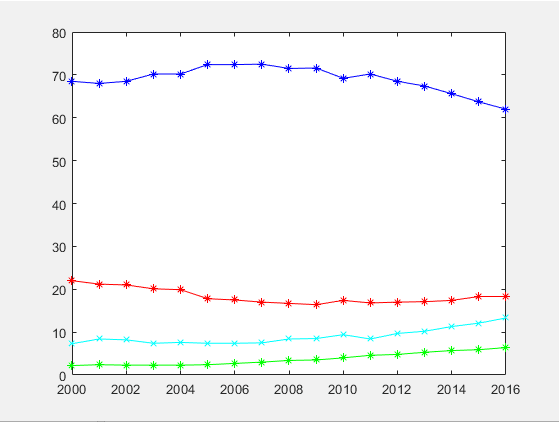
\includegraphics[scale=0.6]{figures/fig1.png}
    \captionsetup{format=hang}
    \caption[煤炭、石油、天然气和一次电力及其他等能源占能源消费总量的比重]{蓝色曲线为煤炭占总能源的比例,红色为石油,绿色为天然气,青色为一次电力及其他能源。}
    \label{fig:nenyuanxiaofeibizhong}
  \end{figure}

  由图 \ref{fig:nenyuanxiaofeibizhong} ,沿 $\mathrm{Y}$ 轴可以分析出以下几点:
  \begin{enumerate}
    \item 煤炭消费占我国能源消费的首要地位,其比例始终居于 $60\%$ 之上。
    \item 石油消费为最主要的辅助能源,其比例一直在 $20\%$ 附近。
    \item 一次电力能源与天然气在总能源中的比例相对较低,大体上低于 $10\%$ 。
  \end{enumerate}

  再沿时间轴可以分析出:
  \begin{enumerate}
    \item 煤炭消费在波动中整体呈现缓步下降趋势,但仍然占据我国能源消费的首要地位。
    \item 石油消费在参考年限中呈稳定趋势,略有波动和下滑。但与一次电力及其他的距离不断拉近。
    \item 一次电力及其他能源和天然气能源消费是呈逐年上升趋势,且天然气的上升速度随年份增加而增加。但所占比例仍然不足。
  \end{enumerate}

  \subsubsection{总结}
  我国的能源消费结构始终为以煤炭消费为主导地位,并以石油消费为主要辅助消费,但也存在天然气、一次电力及其他能源等能源占据市场。能源消费市场呈现 “一超多强” 局面。
  
  天然气和一次电力这样的清洁能源与石油、煤炭消费所占的比重不断拉近,但仍未占据可观消费比例。这说明我国的能源消费结构在不断优化的过程中还有很大的发展空间。
    \subsection{问题 2:碳排放预测模型}

  \subsubsection{碳排放影响因素分析}
    为建立模型,需要对碳排放的影响因素进行分析。根据有关文献,碳排放影响因素一般包括\cite{NCEPU2019}:
    \begin{enumerate}
      \item 人口因素;
      \item 城镇化率;
      \item 经济发展水平:人均 $\mathrm{GDP}$ 或者消除价格波动影响的国内生产总值;
      \item 人均碳排放量;
      \item 能源消费强度:能源消费量与 $\mathrm{GDP}$ 之比;
      \item 能源消费结构:各种能源所占比例,可以用煤炭比例来表示;
      \item 产业结构:三类产业占比,可以用第二产业占比表示;
      \item 国际贸易:出口额占 $\mathrm{GDP}$ 比重。
    \end{enumerate}
    我们选取,如表 \ref{tab:bianliangshuoming} 中变量,作为主要影响因素并确定其计算方法。

  \subsubsection{模型选择}
    由上述可知,影响中国碳排放量的因素繁多,此外碳排放量与影响因素之间不一定线性关系。

    $\mathrm{BP}$ 神经网络实现了一个从输入到输出的映射功能,而理论上一个有无限个隐层节点的神经网络具有实现任何复杂非线性映射的功能。这使得它特别适合于求解内部机制复杂的问题\cite{zhangfaming2016}。

    此外,该模型还拥有自我学习能力,能通过学习大量、正确的实例,提取出规律,完善、改进原有模型。

    总之,由于 $\mathrm{BP}$ 神经网络模型具有较强的自组织、自适应与自学习能力,非线性映射能力,泛化能力以及容错能力\cite{zhoushanshan2018}。我们选用 $\mathrm{BP}$ 神经网络预测模型对我国碳排放量进行预测。

    \begin{table}[htb]
      \centering
      \caption{模型变量说明}
      \begin{tabular*}{0.618\paperwidth}{@{\extracolsep{\fill}}ccccc}
        \toprule[1.5pt]
        &变量 && 计算方法 &\\
        \midrule[1pt]
        &碳排放量 && 各能源按碳排放系数求和(参见 \hyperref[eq:IPCC]{IPCC 方法}) &\\
        &城镇化率 && 城镇人口与总人口比值 &\\
        &$\mathrm{GDP}$ && 各产业生产总值之和 &\\
        &产业结构 && 第二产业与 $\mathrm{GDP}$ 比值 &\\
        &总人口数 && 城乡人口之和 &\\
        &经济发展水平 && $\mathrm{GDP}$ 与人口比值 &\\
        &国际贸易 && 出口额与 $\mathrm{GDP}$ 比值 &\\
        &人均碳排放量 && 碳排放量与总人口比值 &\\
        &能源消费强度 && 能源消费量与 $\mathrm{GDP}$ 比值 &\\
        \bottomrule[1.5pt]
      \end{tabular*}
      \label{tab:bianliangshuoming}
    \end{table}
    \subsection{问题 3:政策建议}
  参见 \hyperref[sec:zhencejianyi]{7 政策建议}。
  \clearpage

  \section{符号说明和模型假设}

  \subsection{符号说明}
    \begin{table}[hb]
      \caption{符号说明}
      \label{tab:fuhaoshuoming}
      \centering
      \begin{tabular*}{0.8\textwidth}{@{\extracolsep{\fill}}ccccc}
        \toprule[1.5pt]
        &符号 && 说明 &\\
        \midrule[1pt]
        &$Y$ && 碳排放总量 &\\
        &$X1$ && 总人口数 &\\
        &$X2$ && $\mathrm{GDP}$ &\\
        &$X3$ && 产业结构 &\\
        &$X4$ && 城镇化率 &\\
        &$X5$ && 经济发展水平 &\\
        &$X6$ && 国际贸易 &\\
        &$X7$ && 人均碳排放量 &\\
        &$X8$ && 能源消费强度 &\\
        \bottomrule[1.5pt]
      \end{tabular*}
    \end{table}

  \subsection{模型假设}
    \begin{enumerate}
      \item 没有外在的、突发的影响或变化,如:能源革命,能源枯竭……即总体碳排放是以某种趋势变化的,总体能源结构稳定;
      \item 限定碳排放主要影响因素在总人口,GDP,产业结构,城镇化率,经济发展水平,国际贸易,人均碳排放量,能源消费强度之中;
      \item 不考虑给定的数据的资金时效性,及给定的 $\mathrm{GDP}$ 已消除价格波动影响。
      \item 使用的数据真实有效。
    \end{enumerate}
  \clearpage

  \section{模型建立及求解}
    \subsection{数据预处理}

  \subsubsection{初始数据计算}

    根据\textbf{问题分析}中问题二的\hyperref[tab:bianliangshuoming]{\textbf{变量计算方法}},我们通过 $\mathrm{Excel}$ 处理\hyperref[ssec:fujian1]{附件 1} 中数据,得到、整理出了 $2000\sim 2016$ 年,碳排放量及其八个变量的具体值。(数据如表 \ref{tab:jutizhi} 所示,具体文件参见 \hyperref[ssec:fujian2]{\textbf{}{附件 2}})
    % Table generated by Excel2LaTeX from sheet 'Sheet1'
    \begin{table}[hb]
      \centering
      \caption{2000--2016 年各变量具体值}
      \resizebox{\textwidth}{!}{
        \begin{tabular}{rrrrrrrrrr}
        \toprule[1.5pt]
        \multicolumn{1}{l}{年份} &
        \multicolumn{1}{l}{碳排放量} & \multicolumn{1}{l}{城镇化率} & \multicolumn{1}{l}{$GDP$} & \multicolumn{1}{l}{产业结构} & \multicolumn{1}{l}{总人口数} & \multicolumn{1}{l}{经济发展水平} & \multicolumn{1}{l}{国际贸易} & \multicolumn{1}{l}{人均碳排放量} & \multicolumn{1}{l}{能源消费强度} \\
        \midrule[1pt]
        2000 & 95528.51053 & 0.362197518 & 100280.1 & 0.455372502 & 126743 & 0.791208193 & 0.205763656 & 0.753718237 & 1.465535036 \\
        2001 & 99939.25859 & 0.376597428 & 110863.2 & 0.447945757 & 127627 & 0.868650051 & 0.198659249 & 0.783057336 & 1.403053493 \\
        2002 & 109314.6759 & 0.390897838 & 121717.4 & 0.444517382 & 128453 & 0.9475637 & 0.221398091 & 0.851009131 & 1.393202615 \\
        2003 & 128517.4696 & 0.405302298 & 137422 & 0.456239903 & 129227 & 1.06341554 & 0.264061795 & 0.994509426 & 1.43414446 \\
        2004 & 149897.5482 & 0.417600086 & 161840.1 & 0.459014175 & 129988 & 1.245038773 & 0.30340441 & 1.153164509 & 1.422892102 \\
        2005 & 171351.2686 & 0.429899966 & 187318.9 & 0.470237654 & 130756 & 1.432583591 & 0.334445697 & 1.310465819 & 1.395315689 \\
        2006 & 187685.8448 & 0.443430102 & 219438.5 & 0.475585642 & 131448 & 1.669393981 & 0.353617073 & 1.427833401 & 1.305454603 \\
        2007 & 203788.9583 & 0.458892446 & 270232.3 & 0.468610155 & 132129 & 2.04521566 & 0.346233962 & 1.542348449 & 1.152497314 \\
        2008 & 207400.2101 & 0.469895032 & 319515.6 & 0.469324815 & 132802 & 2.40595473 & 0.314209827 & 1.56172505 & 1.003428315 \\
        2009 & 217249.6957 & 0.48341701 & 349081.4 & 0.458837681 & 133450 & 2.615821656 & 0.234987295 & 1.627948263 & 0.962887166 \\
        2010 & 229528.7214 & 0.499496611 & 413030.4 & 0.463960522 & 134091 & 3.080224624 & 0.25911614 & 1.711738456 & 0.873175437 \\
        2011 & 248898.1417 & 0.512702713 & 489300.5 & 0.464006883 & 134735 & 3.631576799 & 0.251870987 & 1.847316152 & 0.791012885 \\
        2012 & 254319.7118 & 0.525700866 & 540367.5 & 0.452735037 & 135404 & 3.990779445 & 0.239390785 & 1.878228943 & 0.744193535 \\
        2013 & 261402.5332 & 0.537296431 & 595244.5 & 0.440081513 & 136072 & 4.374481892 & 0.230378273 & 1.921060418 & 0.700406304 \\
        2014 & 262747.8929 & 0.547703645 & 643973.9 & 0.431029581 & 136782 & 4.708031027 & 0.22343095 & 1.920924485 & 0.661216239 \\
        2015 & 261805.7824 & 0.560998676 & 689052.1 & 0.409316364 & 137462 & 5.012673321 & 0.20487101 & 1.904568407 & 0.623907829 \\
        2016 & 260834.8387 & 0.573496973 & 744127.2 & 0.398098605 & 138271 & 5.381657759 & 0.186015634 & 1.886403068 & 0.585678094 \\
        \bottomrule[1.5pt]
        \end{tabular}}%
      \label{tab:jutizhi}%
    \end{table}%

  \subsubsection{数据分类}

    之后我们把数据分类,分别作为 $\mathrm{BP}$ 神经网络的训练数据集和仿真检验数据集。详细如表 \ref{tab:shujufenlei}。

  \subsubsection{数据归一化处理}

    \label{ss2:guiyihua}
    此外,为去除数据量纲,方便数据处理,并使 $\mathrm{BP}$ 神经网络收敛加快,我们将数据集进行了归一化处理\cite{liuzhongqi2010}。计算公式为:
    \[
      y = \frac{x-\min{x}}{\max{x}-\min{x}} \text{式中,$y$ 为归一化后的数据;$x$ 为归一化之前的原始数据。}
    \]
    该过程可由 $\mathrm{MATLAB}$ 中函数 $\mathrm{mapminmax}$ 实现。

    \begin{table}[thb]
      \centering
      \caption{数据分类}
      \begin{tabular*}{0.618\paperwidth}{@{\extracolsep{\fill}}ccccc}
        \toprule[1.5pt]
        &数据集 && 年份 &\\
        \midrule[1pt]
        &训练数据集 && 2000--2014(包括 2014) &\\
        &仿真检验数据集 && 2015--2016(包括 2016) &\\
        \bottomrule[1.5pt]
      \end{tabular*}
      \label{tab:shujufenlei}
    \end{table}
    \subsection{$\mathrm{BP}$ 神经网络结构构建}

  \subsubsection{结构展示}
  最终网络结构示意图如图 \ref{tab:shenjinwanluo} 所示:
  \begin{figure}[hb]
    \caption{神经网络结构图}
    \label{tab:shenjinwanluo}
    \centering
    \def\layersep{2.5cm}
    \def\Layersep{5.0cm}
    \begin{tikzpicture}[shorten >=1pt,->,draw=black!50, node distance=\layersep]
        \tikzstyle{every pin edge}=[<-,shorten <=1pt]
        \tikzstyle{neuron}=[circle,fill=black!25,minimum size=17pt,inner sep=0pt]
        \tikzstyle{input neuron}=[neuron, fill=green!50];
        \tikzstyle{output neuron}=[neuron, fill=red!50];
        \tikzstyle{hidden neuron}=[neuron, fill=blue!50];
        \tikzstyle{annot} = [text width=4em, text centered]

        % Draw the input layer nodes
        \foreach \name / \y in {1,...,8}
        % This is the same as writing \foreach \name / \y in {1/1,2/2,3/3,4/4}
            \node[input neuron, pin=left:输入 $X_\y$] (I-\name) at (0,-\y) {};

        % Draw the hidden layer nodes
        \foreach \name / \y in {2,...,7}
            %\path[yshift=0.5cm]
                \node[hidden neuron] (H-\name) at (\layersep,-\y cm) {};

        % Draw the output layer node
        \node[output neuron, pin={[pin edge={->}]right:输出 $Y$}] (O) at (\Layersep,-4.5 cm) {};

        % Connect every node in the input layer with every node in the
        % hidden layer.
        \foreach \source in {1,...,8}
            \foreach \dest in {2,...,7}
                \path (I-\source) edge (H-\dest);

        % Connect every node in the hidden layer with the output layer
        \foreach \source in {2,...,7}
            \path (H-\source) edge (O);

        % Annotate the layers
        \node[annot,above of=I-1, node distance=1cm] (il) {输入层};
        \node[annot,right of=il] (hl) {隐藏层};
        \node[annot,right of=hl] {输出层};
    \end{tikzpicture}
\end{figure}

  \subsubsection{设计网络输入层和输出层}
    首先设计网络输入、输出层。具体如表 \ref{tab:shurushuchu} 所示:
    \begin{table}[hb]
      \caption{$\mathrm{BP}$神经网络输入、输出层}
      \label{tab:shurushuchu}
      \centering
      \begin{tabular*}{0.8\textwidth}{@{\extracolsep{\fill}}ccccc}
        \toprule[1.5pt]
        &输入层 && 输出层 &\\
        \midrule[1pt]
        &$\mathrm{X_1}$\quad $\mathrm{X_2}$\quad $\mathrm{X_3}$\quad $\mathrm{X_4}$\quad $\mathrm{X_5}$\quad $\mathrm{X_6}$\quad $\mathrm{X_7}$\quad $\mathrm{X_8}$ && $\mathrm{Y}$ &\\
        \bottomrule[1.5pt]
      \end{tabular*}
    \end{table}

  \subsubsection{选取隐含层节点数}

    隐含层节点数的选取是决定神经网络训练精度的关键,过多过少都会有很大影响。

    隐含层节点过多,能有效减少系统误差,但也会导致诸如:网络训练时间延长、训练容易陷入局部极小点的问题。从而降低网络的容错性和范化能力;而隐含层节点数过少,则又可能造成网络性能差或者网络根本不能被训练的问题。

    因此隐含层节点数的选取,我们参考 $\mathrm{Kolmogorov}$ 定理,并采取下列经验公式:
    \[
      J = \sqrt{m+n}+n \text{\qquad 其中 $m$ 为输入节点数,$n$ 为输出节点数,$a$ 的取值范围为 1--10}
    \]
    我们最终选取 6 为隐含层节点数。
    \subsection{$\mathrm{BP}$ 神经网络函数、参数设定}

  具体设定及初始化参见表 \ref{tab:shedingchushihua} 所示:
  \begin{table}[thb]
    \centering
    \caption{函数设定及参数初始化}
    \begin{tabular*}{0.618\paperwidth}{@{\extracolsep{\fill}}ccccc}
      \toprule[1.5pt]
      &函数 && 设定 &\\
      \midrule[1pt]
      &隐层激励函数 && $\mathrm{tansig}$ &\\
      &输出层激励函数 && $\mathrm{logsig}$ &\\
      &网络训练函数 && $\mathrm{traingdx}$ &\\
      &网络性能函数 && $\mathrm{mes}$ &\\
      \midrule[1pt]
      \midrule[1pt]
      &参数 && 初始化 &\\
      \midrule[1pt]
      &期望误差最小值 $\mathrm{err-goal}$ && 0.0000001 &\\
      &最大循环次数 $\mathrm{max-epoch}$ && 5000 &\\
      &修正权值的学习速率 $\mathrm{lr}$ && 0.01 &\\
      \bottomrule[1.5pt]
    \end{tabular*}
    \label{tab:shedingchushihua}
  \end{table}

  \subsubsection{选取激励函数\cite{Sallybin2013}}

    $\mathrm{BP}$ 神经网络通常采用 $\mathrm{Sigmoid}$ 可微函数和线性函数作为网络的激励函数。

    我们选择 $\mathrm{S}$ 型正切函数 $\mathrm{tansig}$ 作为隐层神经元的激励函数。

    而由于网络的输出归一到 $\left[ -1, 1 \right]$ 范围内, 因此预测模型选取 $\mathrm{S}$ 型对数函数 $\mathrm{logsig}$ 作为输出层神经元的激励函数

  \subsubsection{选取训练函数和性能函数}

    $\mathrm{traingdx}$ 该函数运用梯度下降法来训练函数,而且在训练过程中,其学习速率是可变的,训练速度较快,不易陷入局部最小情况。因此我们最终选取 $\mathrm{traingdx}$。

    性能函数我们选取 $\mathrm{BP}$ 神经网络通常采用的 $\mathrm{mex}$ 函数。

  \subsubsection{选取学习速率\cite{zhangfaming2016}}

    学习速率对 $\mathrm{BP}$ 神经网络具有重要影响作用。

    学习速率太小,网络学习缓慢,需要增加训练次数;学习速率太快,容易导致网络不收敛,影响训练的精度。

    我们最终选取学习速率为 $0.01$,最大循环次数为 $5000$ 次。
    \subsection{$\mathrm{BP}$ 神经网络训练与检验}

  \subsubsection{神经网络训练}
    \begin{figure}[htbp]
      \centering
      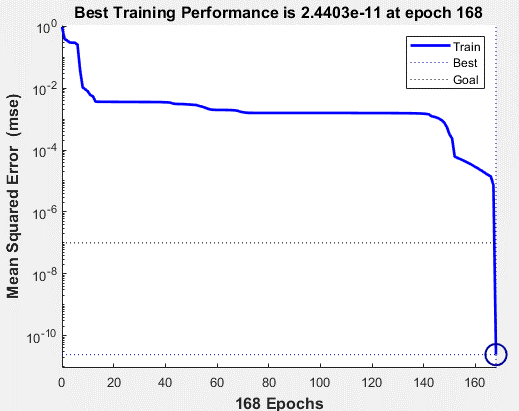
\includegraphics[width=0.618\paperwidth]{figures/muxinxunlian.png}
      \caption{神经网络训练}
      \label{fig:wanluoxunlian}
    \end{figure}
    由图 \ref{fig:wanluoxunlian} 可以看出该 $\mathrm{BP}$ 神经网络通过 168 次重复学习达到期望误差,网络完成训练,BP神经网络模型建立完毕。

  \subsubsection{仿真检验}
    \begin{table}[htb]
      \centering
      \caption{$\mathrm{BP}$神经网络仿真检验}
      \begin{tabular*}{0.618\paperwidth}{@{\extracolsep{\fill}}ccccccccc}
        \toprule[1.5pt]
        &年份 && 真实值 && 预测值 && 相对误差 &\\
        \midrule[1pt]
        &2015 && 261805 && 262060 && 0.0974\% &\\
        &2016 && 260834 && 262650 && 0.6962\% &\\
        \bottomrule[1.5pt]
      \end{tabular*}
      \label{tab:fanzhenjianyan}
    \end{table}
    由图 \ref{tab:fanzhenjianyan} 可知,$\mathrm{BP}$ 神经网络预测的相对误差较小,具有较高的精度和可信度。
  \clearpage

  \section{模型评价}

  \subsection{模型优点}

    \begin{table}[htb]
      \centering
      \caption{模型拟合结果}
      \begin{tabular*}{0.618\paperwidth}{@{\extracolsep{\fill}}ccccccc}
        \toprule[1.5pt]
        &训练次数 && $\mathrm{MES}$ && 平均相对误差 &\\
        \midrule[1pt]
        &168 && $2.4403\times 10^{-11}$ && 0.3968 &\\
        \bottomrule[1.5pt]
      \end{tabular*}
      \label{tab:nihejieguo}
    \end{table}

    由表 \ref{tab:nihejieguo} 可知:
    \begin{enumerate}
      \item 训练次数较少,$\mathrm{BP}$ 神经网络能较快拟合。
      \item 均方根误差 $\mathrm{MES}$ 较小,模型精度较高。
      \item 同时预测平均误差较小,可以较好的预测碳排放量。
    \end{enumerate}
    
    此外,由问题求解可知神经网络模型\cite{zhangfaming2016}:
    \begin{enumerate}
      \item 非常适合求解内部机制复杂、难以清晰暴露内部机理的问题
      \item 自我学习,能随数据不断改善自身。
    \end{enumerate}

  \subsection{模型缺点}
    \begin{enumerate}
      \item 样本数据较少,存在过拟合可能性。
      \item BP神经网络模型不能清晰的反应不同因素对碳排放量的影响程度。
      \item 模型不一定包括了所有影响因素。
    \end{enumerate}
  \clearpage

  \section{模型改进}
  由于 $\mathrm{BP}$ 神经网络像一个 ”黑匣子“ 一样,难以清晰明了地反映出各个因素对碳排放量的影响程度。

  为了确定不同因素对中国碳排放量影响程度的大小,并便于问题三的解决。我们建立了灰色关联度分析模型来对数据进行量化比较分析。
  
  具体通过求解出各个因素对中国碳排放量的关联度,并按关联度大小排序,从而得到得到各影响因素的重要性排序。

  \subsection{灰色关联分析模型简介}
    灰色关联度分析法是一种多因素统计分析方法。它以各因素的样本数据为依据,用灰色关联度来描述各因素间关系的强弱、大小和次序。
    
    若样本数据反映出的两因素变化的态势(方向、大小和速度等)基本一致,则它们之间的关联度较大;反之,关联度较小。
    
    灰色关联度分析对于一个系统发展变化态势提供了量化的度量,这非常适合动态历程分析\cite{guozhonghua2008}。

  \subsection{灰色关联分析模型的建立}

    \subsubsection{确定分析序列}

      在对本问题定性分析的基础上,我们分别以八个因素在 2000--2016 年的\textbf{已归一化}的数据作为八个比较序列。
      \begin{align*}
        \intertext{设 $8$ 个比较序列形成的矩阵为:}
        (X'_1,X'_2,\ldots,X'_8) &= 
        \begin{bmatrix}
          X_1(2000) & X_2(2000) & \cdots & X_8(2000) \\
          X_1(2001) & X_2(2001) & \cdots & X_8(2001) \\
          \vdots & \vdots & \vdots & \vdots \\
          X_1(2016) & X_2(2016) & \cdots & X_8(2016) \\
        \end{bmatrix}
        \intertext{则单个比较序列为:}
        X'_i &= \bigl(X_i(2000),X_i(2001),\dots,X_i(2016)\bigr)^T
        \intertext{当中 $X_i(\text{年份})$ 表示该年份的 $X_i$ 的归一化后的值。}
      \end{align*}

      以中国碳排放量在 2000--2016 年\textbf{已归一化}的数据作为参考数列,参考数量作为理想的比较标准。
      \[
        Y' = [Y(2000),Y(2001),\ldots,Y(2016)]
      \]
      同理,$Y(\text{年份})$ 表示该年份的 $Y$ 值(碳排放量)。

    \subsubsection{计算关联度}
      \begin{enumerate}
        \item 逐个计算每个比较序列对应元素与参考序列对应元素的\textbf{绝对差值}。即:$\Delta_i(k)=|Y(k)-X_i(k)|\qquad (k=2000,\dots,2016\quad i=1,\dots,8)$
        \item 对于任意的 $i,k$ 在其定义范围内的取值,确定绝对差值的最大值和最小值。即:$\Delta_\text{max}$ 和 $\Delta_\text{min}$ 。
        \item 由下式,分别计算每个比较序列对应元素与参考序列对应元素的\textbf{关联系数}。即:
          \[
            \zeta_i(k)=\frac{\Delta_\text{min}+\rho\cdot\Delta_\text{max}}{\Delta_i(k)+\rho\cdot\Delta_\text{max}}
          \]
          其中 $\rho$ 为分辨系数($0<\rho<1$)。\\
          若 $\rho$ 越小,则关联系数间的差异越大,区分能力也就越强。通常取 $\rho$ 为 0.5。
        \item 对各比较序列再分别求其 17 个关联系数的均值,并称该值为\textbf{关联度}\cite{de2013}。即:
          \[
            r_i=\frac{1}{17}\sum_{k=2000}^{2016} \zeta_i(k)
          \]
      \end{enumerate}

    \subsubsection{模型求解}
      利用 $\mathrm{MATLAB}$ 编程实现上述语句。通过带入八个影响因素以及碳排放总量在 2000--2016 年的相关数据,得到其关联度及其排名。如表 \ref{tab:guanlianxu0.5} 所示。
      \begin{table}[htb]
        \centering
        \caption{$\rho=0.5$ 时,各影响因素关联度所求解及排序}
        \begin{tabular*}{0.618\paperwidth}{@{\extracolsep{\fill}}ccccccc}
          \toprule[1.5pt]
          &影响因素 && 关联度 && 排名 &\\
          \midrule[1pt]
          &总人口数 && 0.6746 && 1 &\\
          &$\mathrm{GDP}$ && 0.6066 && 1 &\\
          &产业结构 && 0.3949 && 2 &\\
          &城镇化率 && 0.3949 && 3 &\\
          &经济发展水平 && 0.3949 && 3 &\\
          &国际贸易 && 0.3949 && 3 &\\
          &人均碳排放量 && 0.3949 && 3 &\\
          &能源消费强度 && 0.3949 && 3 &\\
          \bottomrule[1.5pt]
        \end{tabular*}
        \label{tab:guanlianxu0.5}
      \end{table}

      由表 \ref{tab:guanlianxu0.5},我们得到影响因素重要排序。即:
      \[
        \text{总人口}>\textrm{GDP}>\text{其他因素}
      \]

  \section{政策建议}
  \label{sec:zhencejianyi}

  \subsection{建议一}
    我们根据\emph{模型评价与改进}中的灰色预测模型得到了影响因素的重要性排序。结果:
    \[
      \text{总人口}>\textrm{GDP}>\text{其他因素}
    \]
    可见\textbf{总人口}和 \textbf{GDP} 对碳排放量影响最大,其他影响因素之间相差无几。
    
    在其中,\textbf{总人口}一定程度上代表全部人口需要的生产物资、\textbf{GDP} 代表全年所有商品生产的价值总和。需要生产的产品越多,所消耗的能源也越多,因此碳排放量也就越大。
    
    在改革不能自己把自己革命了的前提下,我们提出:
    \begin{enumerate}
      \item 坚持计划生育的基本国策。
      \item 加快中国 $\mathrm{GDP}$ 由高速度增长向高质量发展的经济转型;去杠杆、降产能,稳中求进,积极转变。
      \item 转移城市过剩生产力,帮助农村发展,减少城乡差异;精准扶贫,建设全面小康。
    \end{enumerate}

  \subsubsection{建议二}
    另外,碳排放量在能源消耗一定的情况下,与能源结构、能源利用率有较大关联。
    因此我们提出:
    \begin{enumerate}
      \item 提高化石能源利用率,关闭一些高耗能、高污染、技术落后的小、中型发电厂,加快新技术的研发和推广。
      \item 积极推广绿色能源(风电、水电等)、积极研发新能源,减少对化石能源的依赖。
    \end{enumerate}
  \clearpage

  % 引用文献
  \phantomsection
  \bibliography{ref/math_model}
  \clearpage

  % 附录
  \appendix
  \section{附录}
  \subsection{$\mathrm{BP}$ 代码}
    \lstset{
      basicstyle=\sffamily,
      keywordstyle=\bfseries,
      commentstyle=\rmfamily\itshape,
      stringstyle=\ttfamily
    }
    \begin{lstlisting}[language=MATLAB]
      num=xlsread('student.xls','Sheet1','B2:J18');
      input_train=num(1:14,2:9)';
      output_train=num(1:14,1)';
      input_test=num(14:17,2:9)';
      [inputn,inputps]=mapminmax(input_train);
      [outputn,outputps]=mapminmax(output_train);

      net=newff(inputn,outputn,6);
      net.trainParam.epochs=5000;
      net.trainParam.lr=0.01;
      net.trainParam.goal=0.0000001;
      net=train(net,inputn,outputn);

      inputn_test=mapminmax('apply',input_test,inputps);
      an=sim(net,inputn_test);
      BPoutput=mapminmax('reverse',an,outputps);

      a=[0.573496973;744127.2;0.398098605;138271;5.381657759;0.186015634;1.886403068;0.585678094];
      a=premnmx(a);
      b=sim(net,a);
      c=postmnmx(b,mint,maxt);
    \end{lstlisting}
  \section{附件}

  \subsection{附件 1}
    中国近些年来的一些经济数据\footnote{来源:中国统计年鉴及中国能源统计年鉴}。
    \attachfile{appendix/attachment/fujian1.xlsx}
    \label{ssec:fujian1}

  \subsection{附件 2}
    第一次数据处理:得到 $2000--2016$ 年,八个影响因素的具体值。
    \attachfile{appendix/attachment/fujian2.xlsx}
    \label{ssec:fujian2}

\end{document}